\documentclass[11pt]{article}
\usepackage{subfigure,wrapfig,graphicx,booktabs,fancyhdr,amsmath,amsfonts,appendix,tikz}
\usepackage{bm,amssymb,amsthm,wasysym,color,fullpage,setspace,multirow,placeins}
\usepackage{pgfplots}
\pgfplotsset{compat=1.18}
\usepackage{amsmath,amssymb}
\usepackage{tcolorbox}

% Custom math commands
\newcommand{\vb}{\boldsymbol}
\newcommand{\vbh}[1]{\hat{\boldsymbol{#1}}}
\newcommand{\vbb}[1]{\bar{\boldsymbol{#1}}}
\newcommand{\vbt}[1]{\tilde{\boldsymbol{#1}}}
\newcommand{\vbs}[1]{{\boldsymbol{#1}}^*}
\newcommand{\vbd}[1]{\dot{{\boldsymbol{#1}}}}
\newcommand{\vbdd}[1]{\ddot{{\boldsymbol{#1}}}}
\newcommand{\by}{\times}
\newcommand{\tr}{{\rm tr}}
\newcommand{\cpe}[1]{\left[{#1} \times\right]}
\newcommand{\sfrac}[2]{\textstyle\frac{#1}{#2}}

% Title and Author Information
\title{Advanced Scientific Engineering \\ Homework 3}
\author{Jacob Hands}
\date{October 14, 2024}

\begin{document}
\maketitle

%----------------------------------------
% Section: Exact Solution
%----------------------------------------
\section{Exact Solution}

Given the initial value problem:
\[
\frac{dy}{dt} = -\alpha y, \quad y(0) = 1, \quad \alpha > 0, \quad 0 \leq t \leq T
\]

Step 1: Separate variables and integrate:
\[
\int \frac{1}{y} \, dy = \int -\alpha \, dt
\]
\[
\ln(y) = -\alpha t + C
\]

Exponentiating both sides:
\[
y = e^{-\alpha t + C} = e^C e^{-\alpha t}
\]

Using the initial condition \(y(0) = 1\), we find that \(C_1 = 1\):
\[
y = e^{-\alpha t}
\]

%----------------------------------------
% Section: Forward Euler Method
%----------------------------------------
\section{Derive the Update Equation Using Forward Euler}

We know that for the Forward Euler method:
\[
u^{n+1} = u^n + \Delta t \, f(u^n, t^n)
\]
For our equation \(\frac{dy}{dt} = -\alpha y\), this becomes:
\[
\frac{y^{n+1} - y^n}{\Delta t} \approx -\alpha y^n
\]

Rearranging to find \(y^{n+1}\):
\[
y^{n+1} = y^n (1 - \alpha \Delta t)
\]

\begin{tcolorbox}
\[
y^{n+1} = y^n (1 - \alpha \Delta t)
\]
\end{tcolorbox}

%----------------------------------------
% Section: Stability Condition
%----------------------------------------
\section{Stability Condition for Forward Euler}

We derived that:
\[
y^{n+1} = y^n (1 - \alpha \Delta t)
\]

For stability, we require \(|1 - \alpha \Delta t| \leq 1\).

### Upper bound:
\[
1 - \alpha \Delta t \leq 1 \quad \Rightarrow \quad -\alpha \Delta t \leq 0 \quad \Rightarrow \text{always passes since } -\alpha \Delta t \text{ is always negative.}
\]

### Lower bound:
\[
1 - \alpha \Delta t \geq -1 \quad \Rightarrow 2 \geq \alpha \Delta t \quad \Rightarrow \Delta t \leq \frac{2}{\alpha}
\]

Thus, the stability condition is:
\[
\Delta t \leq \frac{2}{\alpha}
\]

\begin{figure}[!ht]
    \centering
    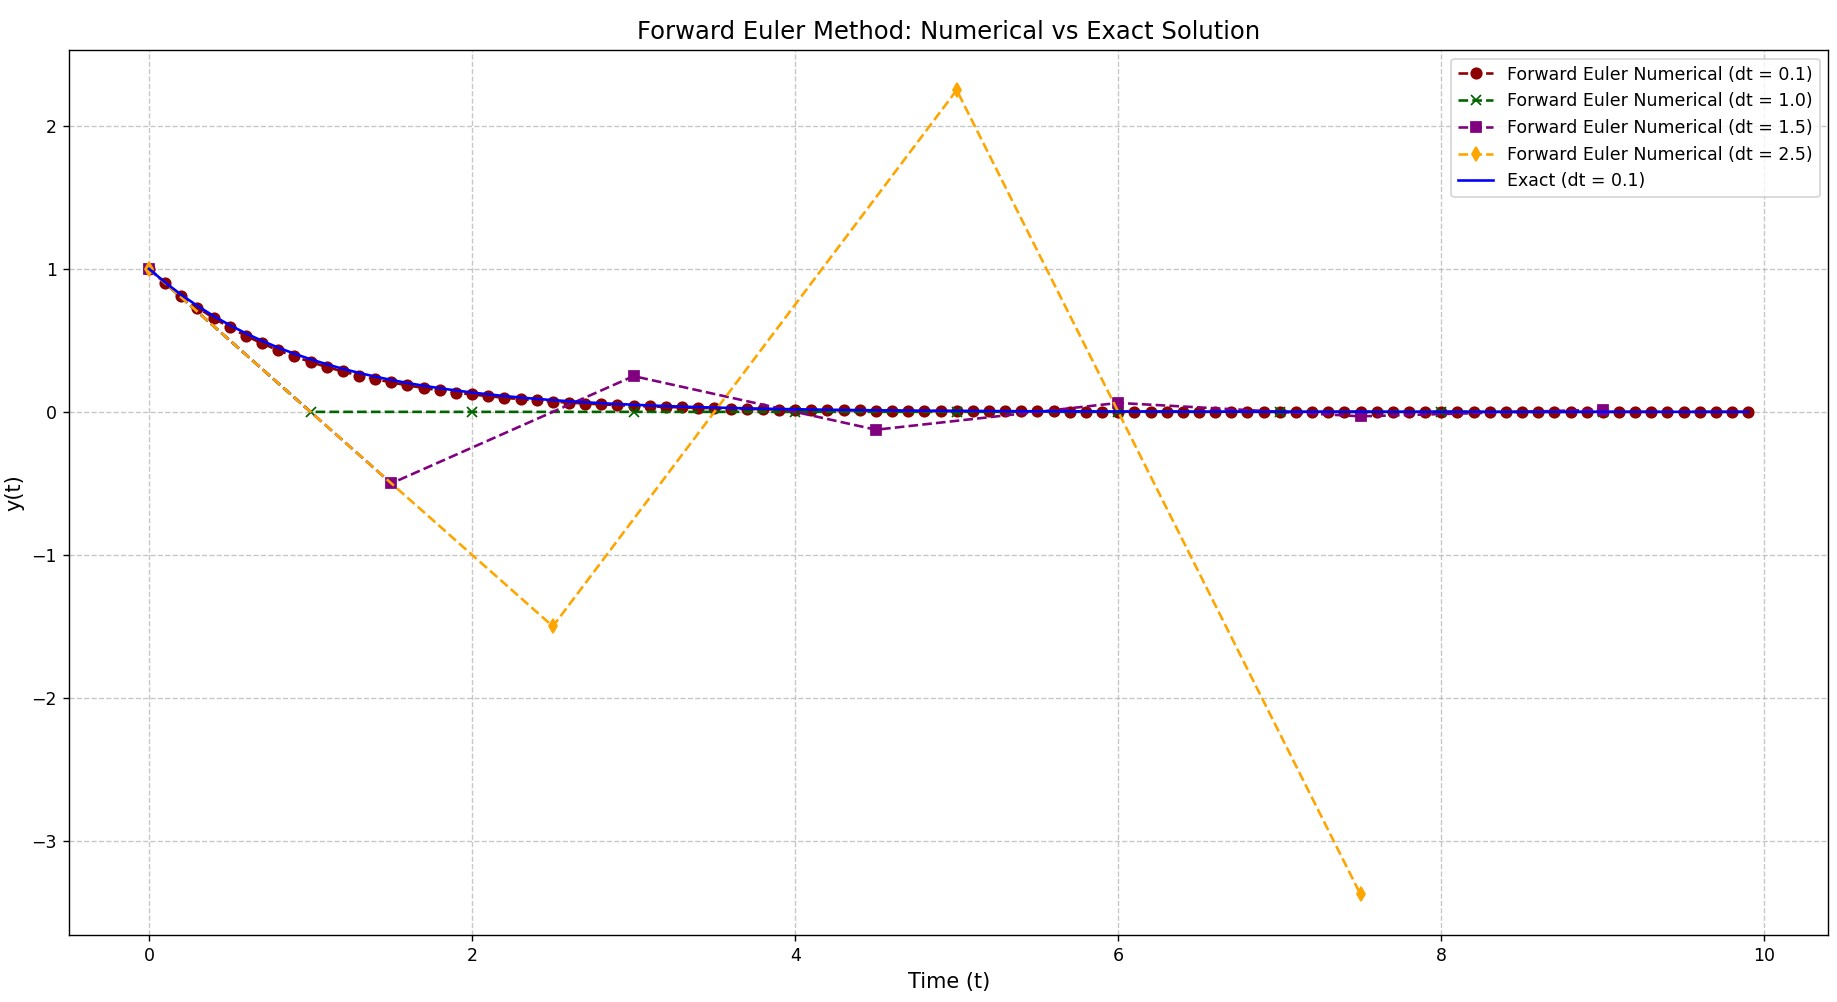
\includegraphics[width= 1 \textwidth]{images/Forward Euler.jpg}
    \caption{Forward Euler Numerical vs Exact Solution}
    \label{fig:3}
    \end{figure}
    \FloatBarrier

%----------------------------------------
% Section: Backward Euler Method
%----------------------------------------
\section{Derive the Update Equation Using Backward Euler}

For Backward Euler, we update using:
\[
y^{n+1} = y^n + \Delta t \, f(u^{n+1})
\]
For the equation \(\frac{dy}{dt} = -\alpha y\):
\[
\frac{y^{n+1} - y^n}{\Delta t} = -\alpha y^{n+1}
\]
Rearranging:
\[
y^{n+1} - y^n = -\Delta t \alpha y^{n+1}
\]
\[
y^{n+1}(1 + \Delta t \alpha) = y^n
\]
Finally, solving for \(y^{n+1}\):
\[
y^{n+1} = \frac{y^n}{1 + \Delta t \alpha}
\]

\begin{tcolorbox}
\[
y^{n+1} = \frac{y^n}{1 + \Delta t \alpha}
\]
\end{tcolorbox}

\begin{figure}[!ht]
    \centering
    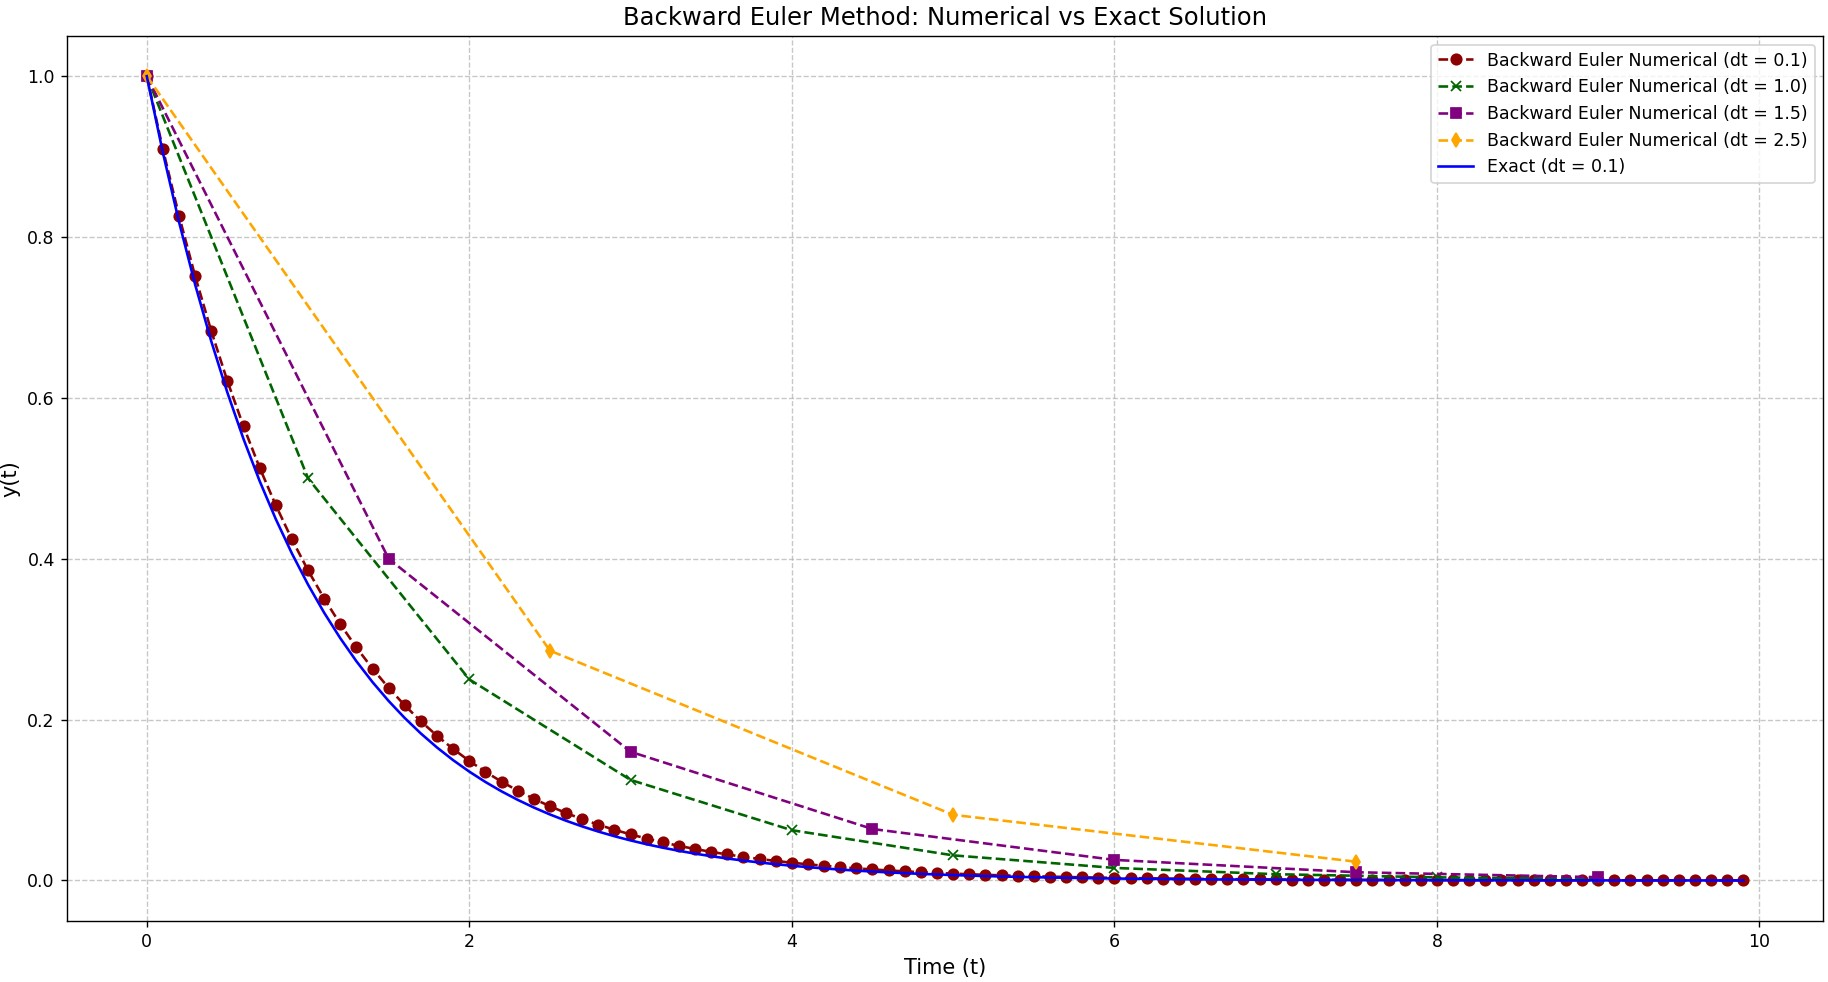
\includegraphics[width= 1 \textwidth]{images/Backward Euler.jpg}
    \caption{Backward Euler Numerical vs Exact Solution}
    \label{fig:2}
  \end{figure}
  \FloatBarrier
%----------------------------------------
% Section: Trapezoidal Method
%----------------------------------------
\section{Derive the Update Equation Using Trapezoidal Method}

For the Trapezoidal method, we use the average of the function at the previous and next time steps:
\[
y^{n+1} = y^n + \frac{\Delta t}{2} \left( f(y^n) + f(y^{n+1}) \right)
\]
For the equation \(\frac{dy}{dt} = -\alpha y\):
\[
y^{n+1} - y^n = \frac{-\alpha \Delta t}{2} (y^n + y^{n+1})
\]
Rearranging:
\[
y^{n+1}(1 + \frac{\alpha \Delta t}{2}) = y^n \left(1 - \frac{\alpha \Delta t}{2}\right)
\]
Finally, solving for \(y^{n+1}\):
\[
y^{n+1} = y^n \left(\frac{1 - \frac{\alpha \Delta t}{2}}{1 + \frac{\alpha \Delta t}{2}}\right)
\]

\begin{tcolorbox}
\[
y^{n+1} = y^n \left(\frac{1 - \frac{\alpha \Delta t}{2}}{1 + \frac{\alpha \Delta t}{2}}\right)
\]
\end{tcolorbox}


\begin{figure}[!ht]
    \centering
    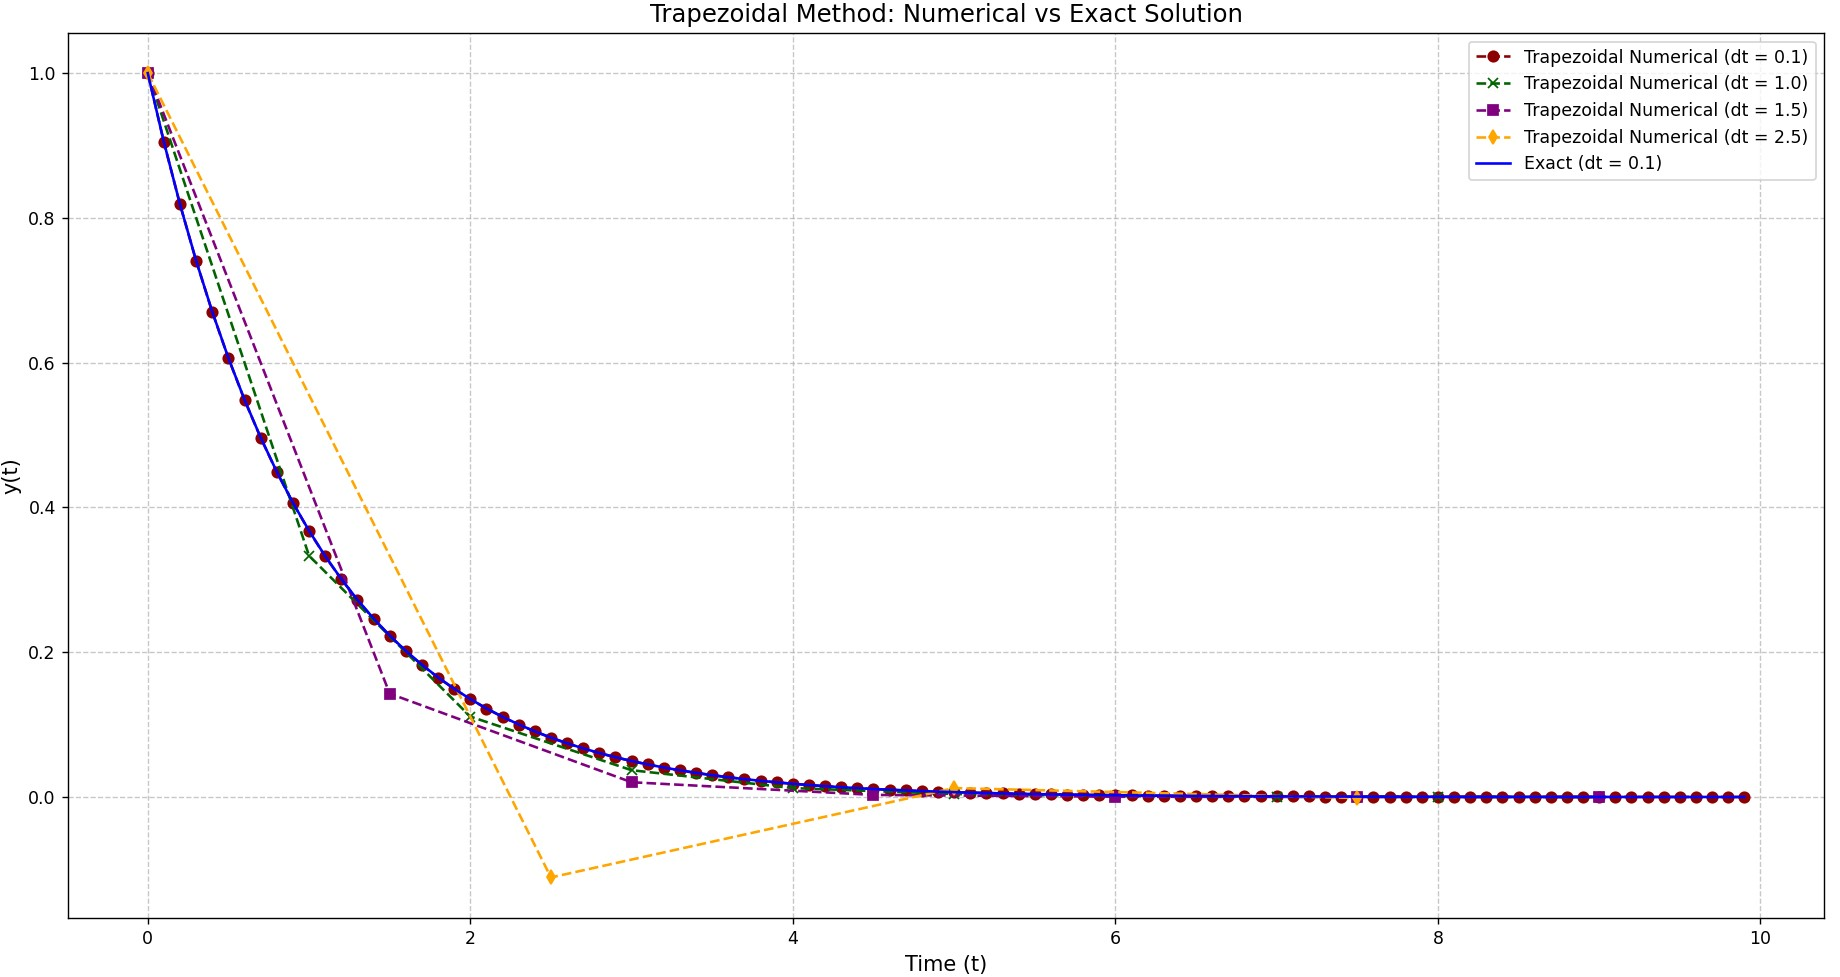
\includegraphics[width= 1 \textwidth]{images/Trapezoidal method.jpg}
    \caption{Trapezoidal Method Numerical vs Exact Solution}
    \label{fig:1}
  \end{figure}
  \FloatBarrier


\end{document}
